\documentclass[conference]{IEEEtran}

\usepackage[T1]{fontenc}
\usepackage{cite}
\usepackage{amsmath}
\usepackage{graphicx}
\usepackage{booktabs}
\usepackage{tabularx}
\usepackage{stfloats}
\usepackage{placeins}
\usepackage{url}
\usepackage[hidelinks]{hyperref}
\urlstyle{same}

\newcolumntype{Y}{>{\raggedright\arraybackslash}X}
\newcolumntype{L}[1]{>{\raggedright\arraybackslash}p{#1}}

\begin{document}
\bstctlcite{IEEEexample:BSTcontrol}

\title{Learning Based Interventions for Rework and Repeated Decisions in Business Processes}
\author{\IEEEauthorblockN{Mridankan Mandal, Aditya Pachauri and Dhannu Ram Meena}
\IEEEauthorblockA{IIB2024017, IIB2024001 and IIB2024033\\
Group Number 7}}
\maketitle

\begin{abstract}
Event logs show where work repeats. They do not reveal what another intervention would have caused. This makes it difficult to test whether sequential control adds value beyond supervised prediction when repeated work competes for shared capacity. We study this question in four simulators of document requests, incomplete applications, physical repair and repeated loan offers. The evaluation compares deterministic rules, four machine learning families and four reinforcement learning methods under matched random draws. Across three random seeds, focused controllers reduce claims queue time by 11.25\% and manufacturing tail wait by 7.30\% against Regression controls. In SimBank, forecast informed conservative Q learning avoids 5.75 refusals per 100 cases, a 22.95\% reduction without a confirmed profit change. The BPISim episodic controller saves 0.11\% of elapsed time. Its interval crosses zero. Ablations show that congestion state, accrued waiting and reward design explain the useful gains. Specialist effects remain simulation assumptions.
\end{abstract}

\begin{IEEEkeywords}
business process simulation, rework, loops, repeated decisions, machine learning, reinforcement learning
\end{IEEEkeywords}

\section{Introduction}

A missing document can return a claim to review \cite{levich}. An incomplete application can enter another review \cite{bpi}. A failed inspection can send a part through another repair \cite{production}. Such loops make repeated work compete with new cases for limited resources \cite{lopez,shoush}. Repeated loan offers create a related decision problem \cite{simbank}. The action changes the next outcome but does not represent corrective rework.

Recorded event logs show observed paths but do not reveal outcomes under actions not taken \cite{simbank,scope}. Process simulation can expose such alternative outcomes under declared assumptions. It also lets policies face the same arrivals, case difficulty and repeat draws \cite{simbank}. Fig.~\ref{fig:bpmn} shows the four process models. The first three contain corrective returns with shared resources. SimBank contains repeated offers without a shared reviewer queue.

Stochastic process models learn data dependent behavior from event logs \cite{mannhardt,horvath}. Prescriptive methods recommend interventions for running cases under uncertainty or resource limits \cite{shoush,scope}. The closest methods leave a practical gap for this setting. They do not show across several repeat mechanisms whether sequential control improves a strong supervised policy when cases compete for capacity and repeat outcomes are constrained. A gain over FIFO does not answer this question. We test the stronger comparison between supervised machine learning and forecast informed control.

The work makes three contributions:
\begin{itemize}
\item We construct three log grounded simulators that connect corrective returns to shared queues. We add SimBank as an independent repeated decision setting.
\item We compare deterministic rules, four machine learning methods and four reinforcement learning controllers under one split and seed protocol.
\item We isolate when sequential control helps. Focused policies improve claims queues, manufacturing tail wait and repeated loan refusals. The BPISim result shows the boundary when the controlled stage forms little of total elapsed time.
\end{itemize}

\begin{figure*}[!t]
\centering
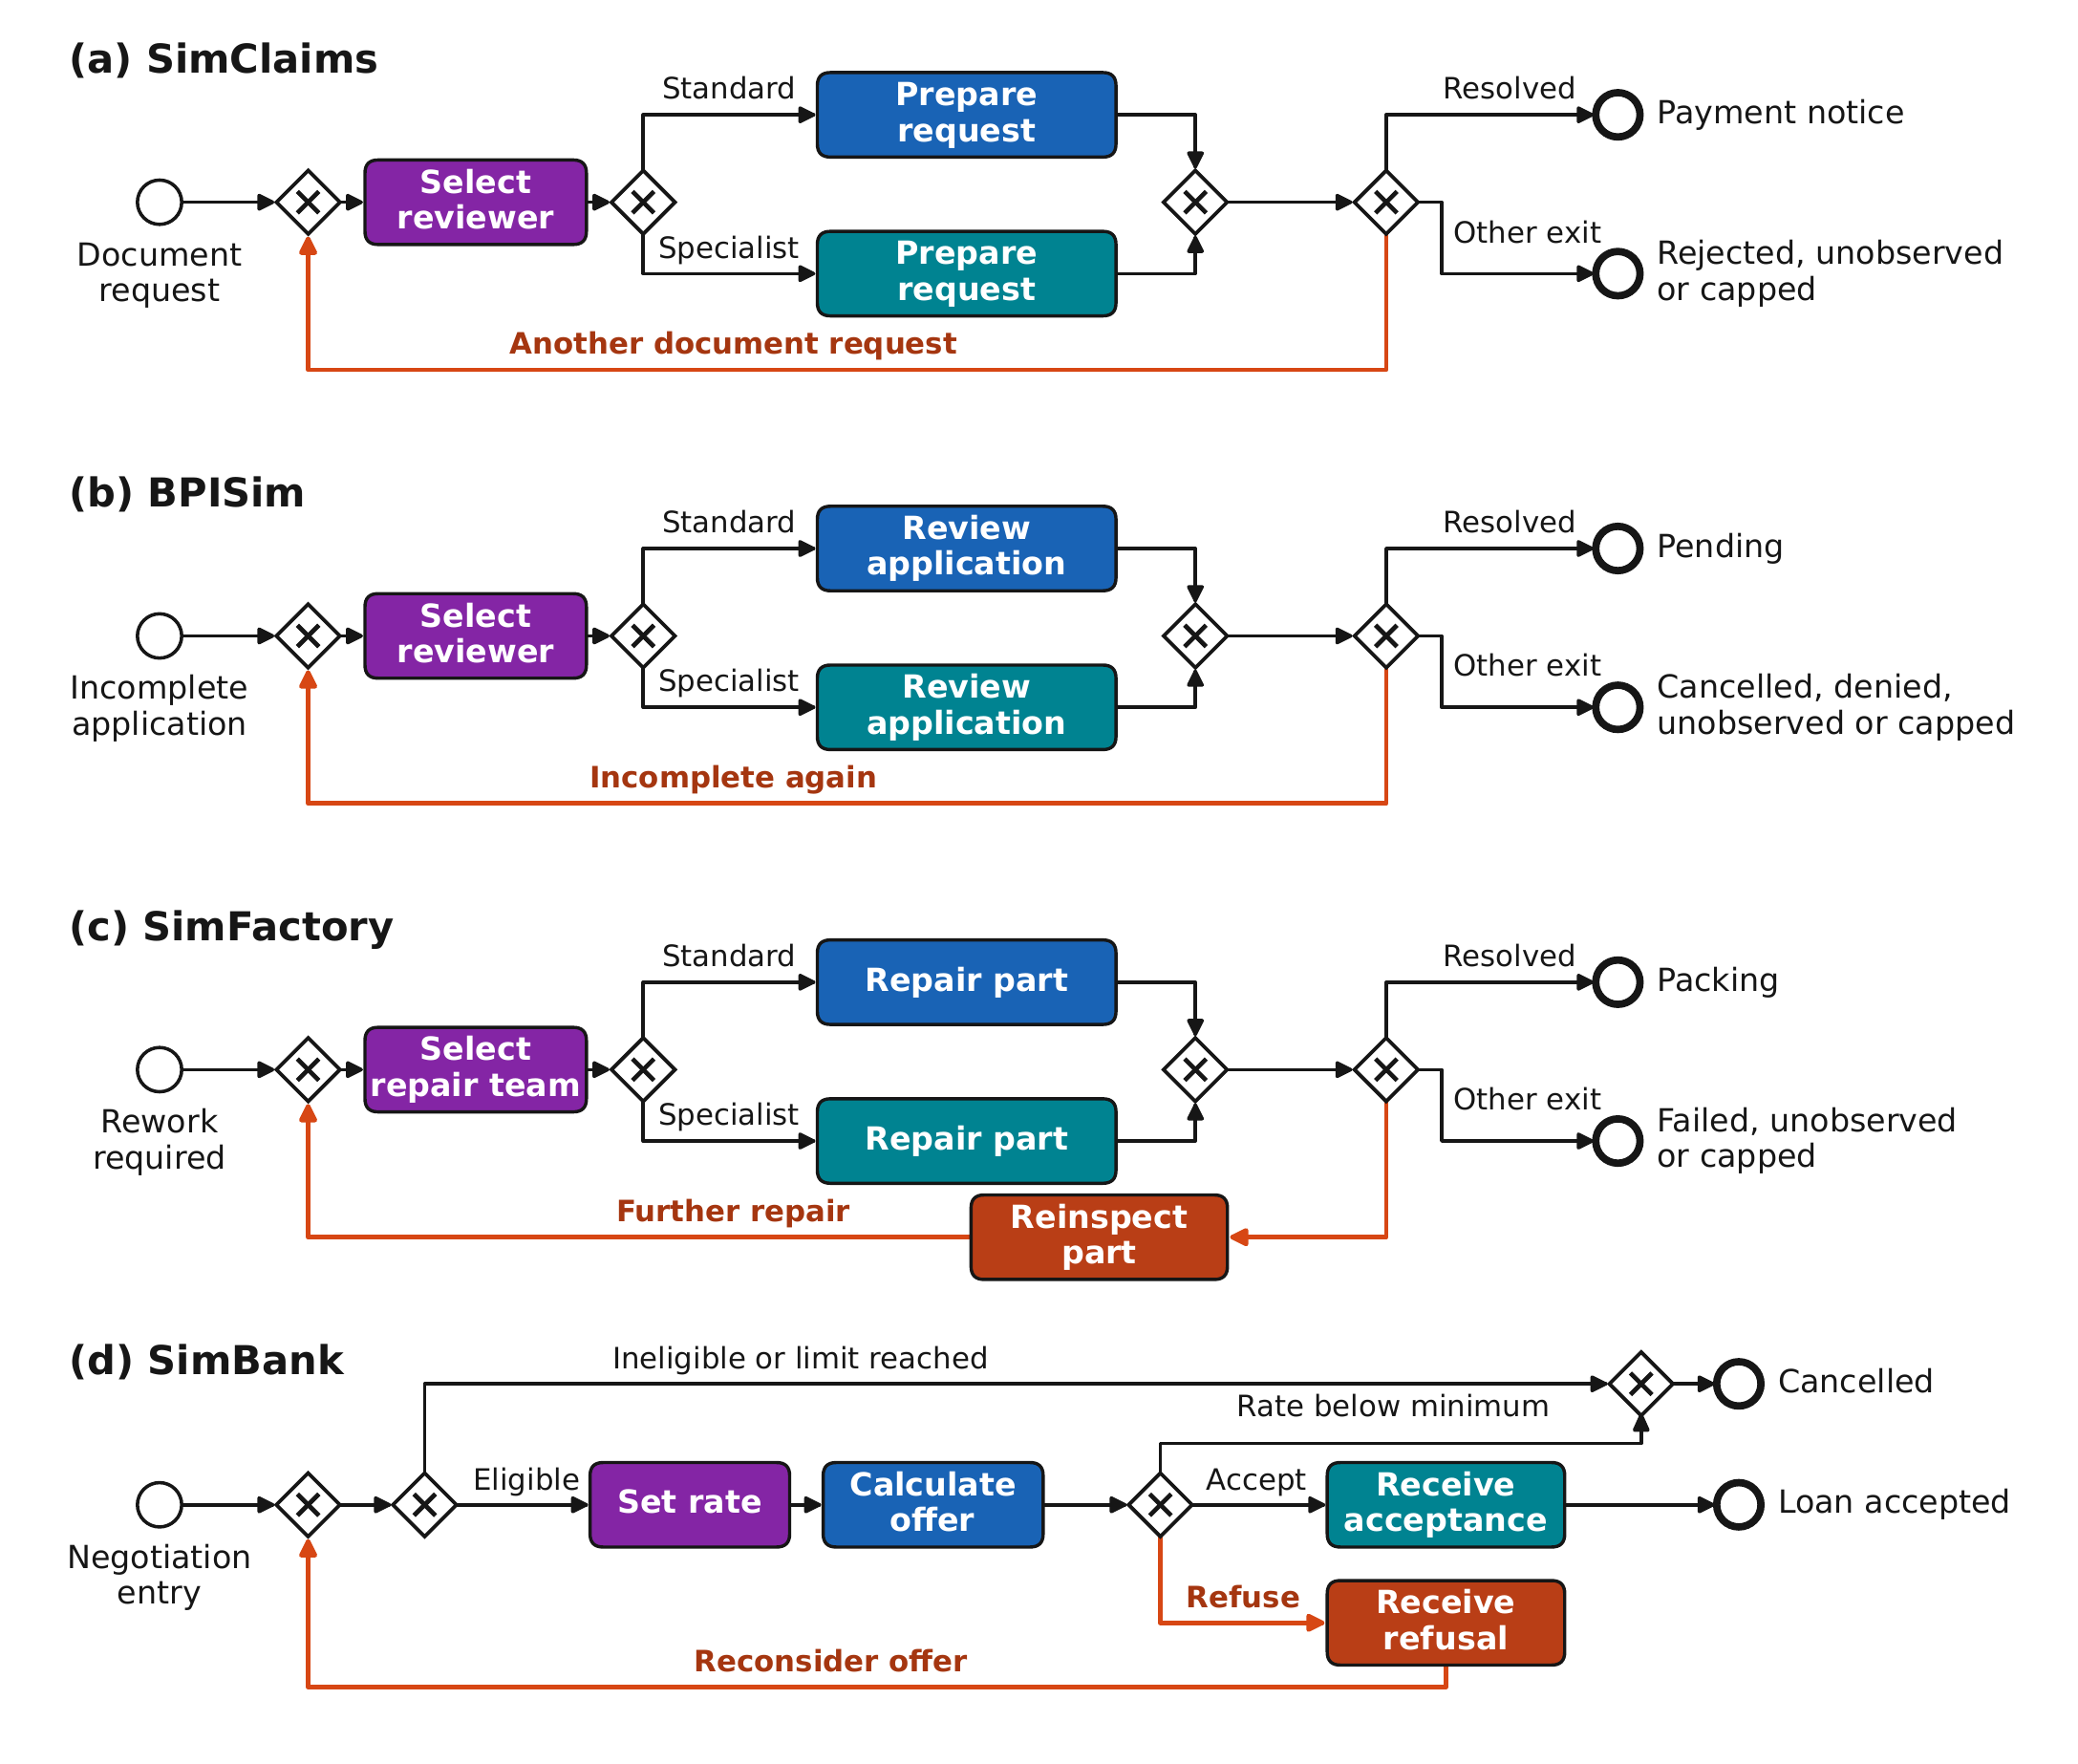
\includegraphics[width=.97\textwidth]{img/fig01_corrective_loops.png}
\caption{BPMN models of repeated work in the four simulators.}
\label{fig:bpmn}
\end{figure*}

\section{Related Work}

Observed process behavior can be represented with data dependent transition weights learned from event logs \cite{mannhardt}. Stochastic process trees can also represent choice, loop and timing parameters \cite{horvath}. Differentiated resource models can improve process simulation accuracy \cite{lopez}. These methods estimate process behavior. They do not evaluate which intervention should receive scarce capacity when repeated work occurs.

Prescriptive monitoring moves from prediction to action. Running cases can be ranked using predicted outcomes, uncertainty, intervention effects and available resources \cite{shoush}. Sequential intervention decisions can be aligned through causal learners and backward induction \cite{scope}. These approaches prescribe interventions for running cases. Our routing domains add shared corrective queues where one action can change the delay faced by later cases.

Known intervention outcomes can be generated in a loan process with parallel activities and loops through SimBank \cite{simbank}. This capability supports direct policy evaluation instead of relying only on logged action estimates. Off policy estimates may otherwise have high variance when the evaluated policy differs from the logging policy \cite{ope}. The released SimBank simulator evaluates cases independently \cite{simbank}. We retain that mechanism as a repeated decision benchmark and use log grounded routing simulators for shared capacity.

Existing work does not provide a matched comparison between supervised prediction and sequential control across distinct repeat mechanisms. Such a comparison must preserve the same process model, forecasts, random draws and operating limits. We address this limitation by separating broad algorithm screening from focused controllers that use congestion, accrued wait or repeated offer history.

\section{Methodology}
\label{sec:methodology}

\subsection{Process Models and Data}

The routing simulators use insurance claims, loan applications and manufacturing event logs. Table~\ref{tab:data} connects each source to its repeated episode and intervention. Fig.~\ref{fig:bpmn} shows the corresponding paths with BPMN 2.0 notation \cite{bpmn}. Each simulation starts when a case becomes eligible for repeated work and ends at resolution, a negative outcome, an unobserved exit or an attempt limit.

\begin{table*}[!tb]
\caption{Simulator data and intervention summary.}
\label{tab:data}
\centering\footnotesize
\setlength{\tabcolsep}{5pt}
\renewcommand{\arraystretch}{1.12}
\begin{tabularx}{\textwidth}{@{}L{.68in}L{1.55in}L{.61in}Y Y@{}}
\toprule
Simulator & Source data & Cases & Repeated episode & Decision \\
\midrule
SimClaims & Insurance claim events \cite{levich} & 5,131 & Later document request & Standard or specialist preparation \\
BPISim & Loan application events \cite{bpi} & 31,509 & Incomplete Review Marker & Standard or specialist review \\
SimFactory & Manufacturing events \cite{production} & 225 & Repair after reinspection & Standard or specialist repair \\
SimBank & Synthetic loan negotiations \cite{simbank} & 100,000 & Offer after refusal & Rate for the next offer \\
\bottomrule
\end{tabularx}
\end{table*}

SimClaims groups adjacent document requests into one attempt. A later request starts a new attempt. BPISim starts an attempt at each Incomplete Review Marker and measures review work from matched lifecycle events. SimFactory requires reinspection before another repair. These definitions prevent adjacent log events from being counted as separate corrective cycles.

Cases follow a roughly 70/30 chronological train and test boundary. The split is fixed before eligibility filtering, so the small manufacturing group can differ from that ratio. First and later attempts have separate outcome distributions. Work and residual time are sampled together from matching historical records. These simulators preserve the selected repeat structure and empirical timing distributions. They do not reproduce every path in the source log.

\subsection{Actions and Intervention Assumptions}

The three routing domains use two standard servers and one specialist. A workload contains 80 cases. Ten specialist slots are available. Specialist service is slower but prevents 25\% of potential repeats. Case difficulty affects return risk. These are declared scenario assumptions because the logs do not identify the causal effect of specialist service.

SimBank uses the released 100,000 case family. A policy chooses an interest rate from 5\% to 9\% for at most three offers. Customer response, duration and profit follow the native simulator \cite{simbank}. Compared policies share customer draws. Cases remain independent and do not compete for a reviewer.

\subsection{Learning Methods}

Regression denotes task matched logistic, ridge and Poisson models. Logistic regression predicts binary returns. Poisson regression predicts counts and ridge regression predicts continuous time or effort. We compare this family with Random Forest \cite{rf}, CatBoost \cite{cat} and XGBoost \cite{xgb}. Routing models use attempt history, case difficulty and the candidate action to forecast return risk, work and elapsed time. SimBank models use loan attributes and offer history to forecast refusal, effort and profit.

Deterministic controls use FIFO or the released bank rule. Supervised routing combines forecasts with current waits and remaining specialist slots. The reinforcement learning screen includes Q learning \cite{q}, fitted Q, CQL \cite{cql} and PPO \cite{ppo}. Q learning and PPO collect simulator experience. Fitted Q and CQL learn from replay generated by randomized policies. Within each seed, every controller receives the same validation selected forecasts. This keeps the controller comparison separate from forecaster selection.

After screening, focused routing experiments use Regression because it gives the best mean supervised result in all three routing domains. Episodic policy search adjusts its action score with process state. For state $s$, the specialist action is
\begin{equation}
 a(s)=\mathbf{1}\{g_{\mathrm{ML}}(s)+\theta^{\mathsf{T}}\phi(s)>0\}.
\end{equation}
Here $a(s)=1$ assigns specialist service, $g_{\mathrm{ML}}$ is the regression score and $\theta$ is learned from complete workload returns. The state vector $\phi(s)$ contains congestion, repeat stage, progress and remaining specialist capacity. SimFactory also includes accrued wait. Validation keeps a controller only when it satisfies the domain limit. Else, it retains Regression. BPISim reports the same episodic controller as a sensitivity analysis. Validation retains Regression in every seed.

SimBank uses a Regression based dynamic planner as the focused control. The candidate is CQL with forecast features and a reward that combines profit, refusals and cancellations. This comparison tests whether offline control can reduce repeated refusals without a clear loss of native profit.

\subsection{Experimental Setup}

Three random seeds are generated from master seed 17. Predictor fitting, calibration, policy training, validation and testing use separate random streams. Validation fixes model and policy choices before the held out test. Compared policies share arrivals, case attributes and outcome draws.

The common routing screen evaluates 256 workloads per seed. Focused routing uses 384 workloads per seed. SimBank evaluates 30,000 paired cases per seed. Queue time starts when service is ready. Manufacturing tail wait is the mean queue time of the eight longest waiting cases in a workload. Extra attempts are the number of corrective attempts made after the initial attempt, measured per 100 cases. SimBank repeat refusals exclude the first refusal in a case.

Tables report mean $\pm$ standard deviation across seeds. Paired 95\% intervals resample seeds and matched test units. Focused queue and tail comparisons require a 5\% gain with at most 0.50 additional attempts per 100 cases. BPISim targets a 30 minute elapsed time gain. SimBank targets one fewer refusal per 100 cases with no more than 0.5\% profit loss. These limits are fixed before test evaluation.

\section{Results}
\label{sec:results}

Table~\ref{tab:screening} reports the common algorithm screen. Routing uses FIFO as the deterministic reference. SimBank uses its released bank rule. Fig.~\ref{fig:benchmark} shows the same primary outcomes as gains over these references. A positive bar means less waiting in the routing domains or more profit in SimBank.

\begin{figure*}[!t]
\centering
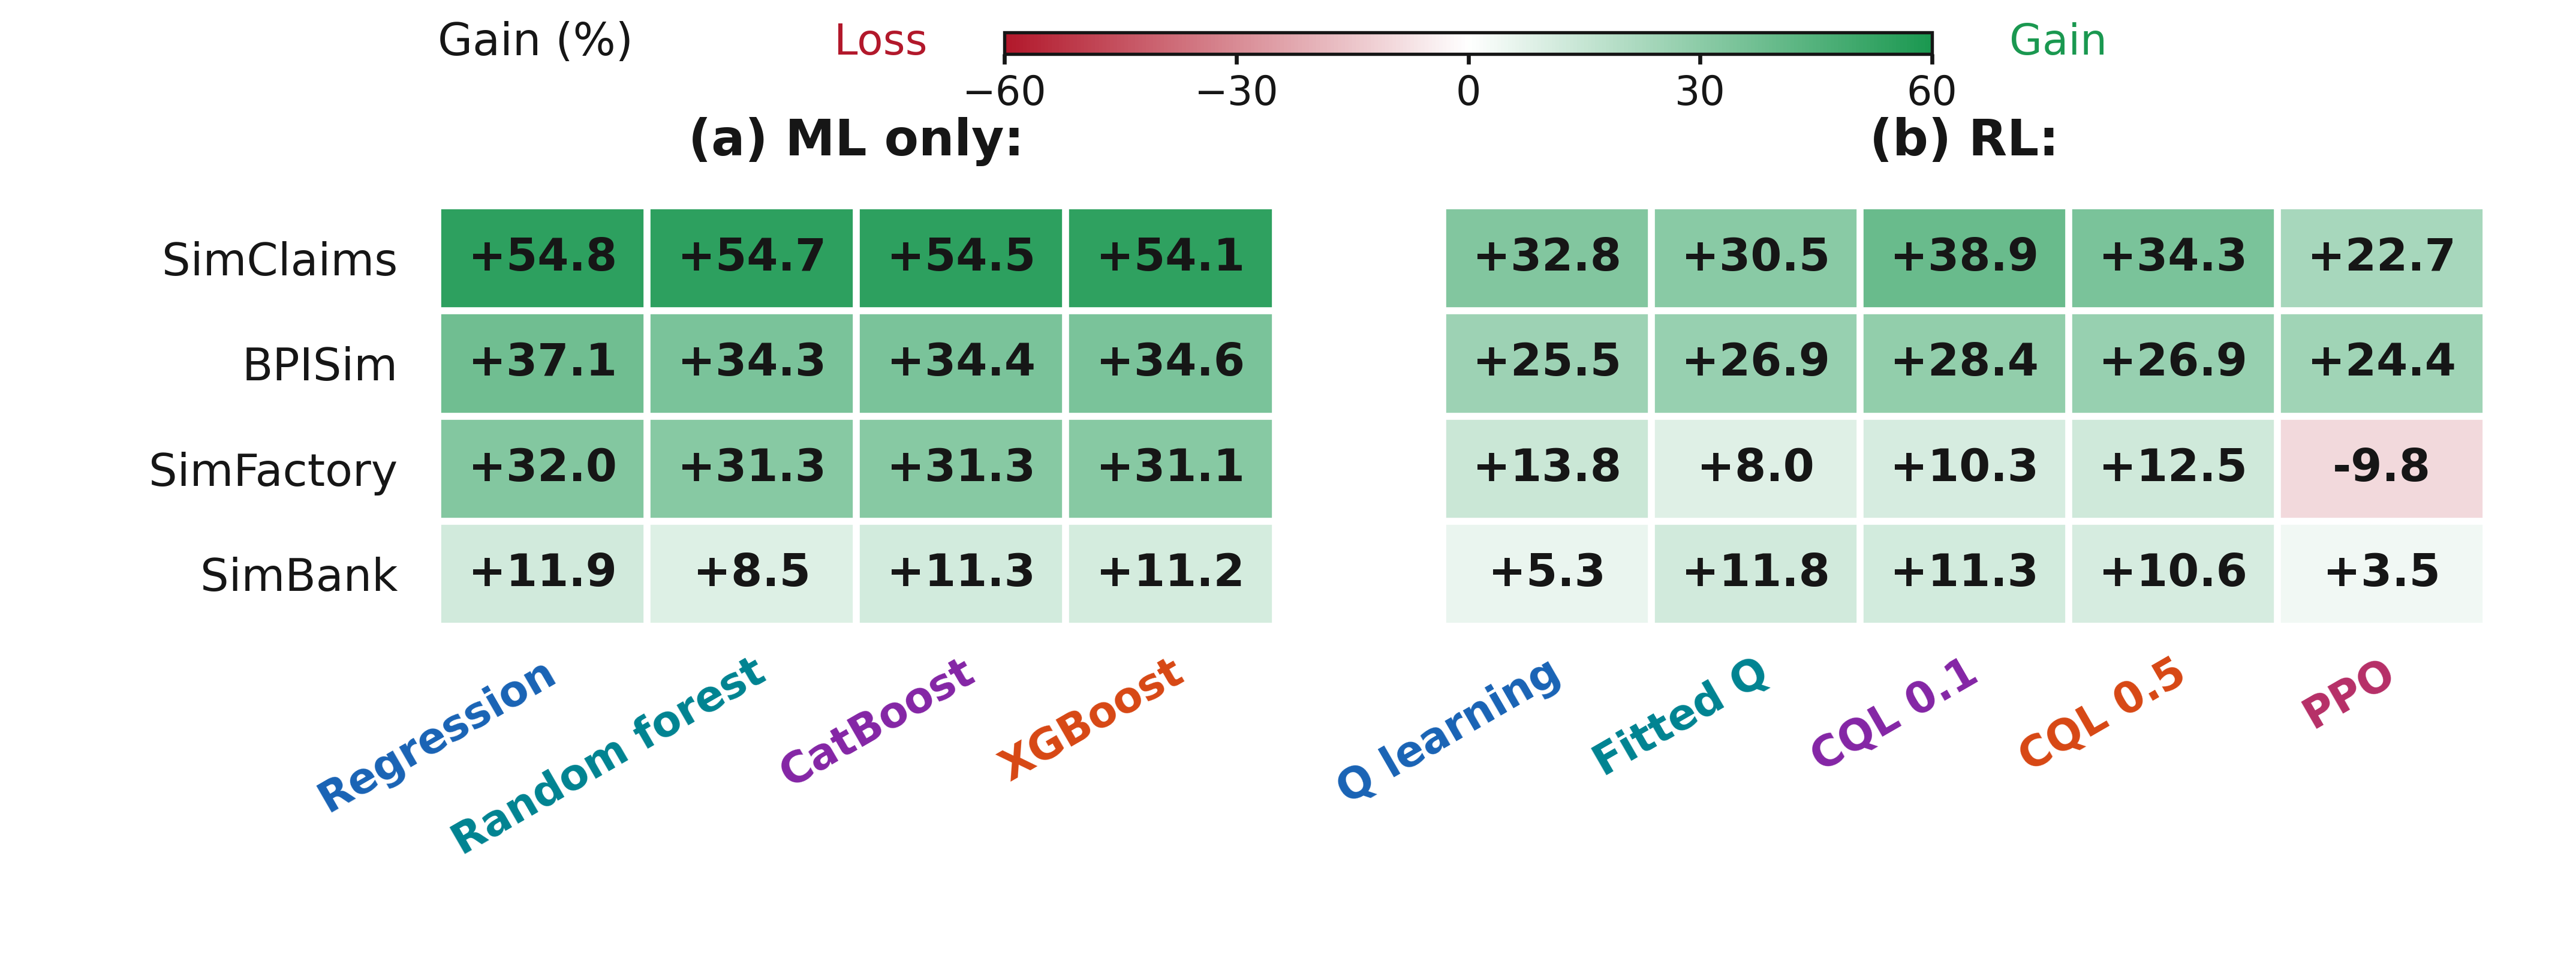
\includegraphics[width=\textwidth]{img/fig02_policy_gains.png}
\caption{Primary metric gains over FIFO for routing and over the bank policy for SimBank. Positive values mean lower waiting or higher profit.}
\label{fig:benchmark}
\end{figure*}

\begin{table*}[!tbp]
\caption{Common benchmark results across model and controller families.}
\label{tab:screening}
\centering\footnotesize
\setlength{\tabcolsep}{4pt}
\renewcommand{\arraystretch}{1.14}
\begin{tabularx}{\textwidth}{@{}Yrrrrr@{}}
\toprule
Method & Claims wait $\downarrow$ & BPI wait $\downarrow$ & Factory tail $\downarrow$ & Bank profit $\uparrow$ & Bank refusals $\downarrow$ \\
\midrule
\multicolumn{6}{@{}l}{\textit{Deterministic reference}} \\
FIFO / bank rule & $122.9\pm3.1$ & $55.9\pm0.5$ & $1051.0\pm25.4$ & $3378\pm45$ & $15.9\pm0.1$ \\
\midrule\multicolumn{6}{@{}l}{\textit{ML only}} \\
Regression & $55.6\pm1.3$ & $35.2\pm1.0$ & $714.4\pm19.3$ & $3780\pm83$ & $24.3\pm2.9$ \\
Random Forest & $55.7\pm2.9$ & $36.8\pm0.9$ & $722.2\pm24.8$ & $3667\pm60$ & $26.8\pm2.2$ \\
CatBoost & $55.9\pm2.9$ & $36.7\pm0.8$ & $722.2\pm25.7$ & $3759\pm109$ & $23.3\pm3.3$ \\
XGBoost & $56.4\pm3.5$ & $36.6\pm1.0$ & $724.2\pm30.7$ & $3756\pm99$ & $23.6\pm2.4$ \\
\midrule\multicolumn{6}{@{}l}{\textit{RL with best validation selected forecaster}} \\
Q learning & $82.6\pm3.7$ & $41.7\pm0.8$ & $906.5\pm53.6$ & $3557\pm129$ & $14.8\pm0.4$ \\
Fitted Q & $85.4\pm11.2$ & $40.9\pm1.9$ & $967.3\pm48.7$ & $3778\pm79$ & $20.5\pm1.5$ \\
CQL $\alpha{=}0.1$ & $75.1\pm11.6$ & $40.0\pm2.5$ & $942.5\pm152.4$ & $3762\pm47$ & $17.9\pm2.0$ \\
CQL $\alpha{=}0.5$ & $80.7\pm28.6$ & $40.9\pm1.2$ & $919.9\pm242.2$ & $3736\pm60$ & $16.4\pm1.7$ \\
PPO & $95.1\pm29.8$ & $42.3\pm3.5$ & $1153.9\pm29.8$ & $3496\pm57$ & $34.0\pm0.2$ \\
\bottomrule
\end{tabularx}
\par\smallskip
\begin{minipage}{\textwidth}\footnotesize
Means $\pm$ SD across three random seeds. Routing columns report minutes. SimBank ML rows use refusal aware planners. RL rows use the best forecast family selected on validation, not every ML and RL pairing. Routing uses 256 workloads per seed. SimBank uses 30,000 cases per seed.
\end{minipage}
\end{table*}


\subsection{Model and Controller Screening}

All four supervised families reduce routing wait by a large margin against FIFO (Table~\ref{tab:screening}). Regression gives the lowest mean in SimClaims, BPISim and SimFactory. The differences among supervised models are small compared with their gains over FIFO. This result supports the use of Regression as the focused control.

Generic reinforcement learning does not improve the best supervised routing mean. CQL is the strongest RL family for SimClaims and SimFactory, yet its mean wait remains above Regression. PPO is also less stable across the routing domains. SimBank shows a different tradeoff. Fitted Q nearly matches Regression profit. Q learning produces fewer refusals than the bank rule but its profit is lower. Fig.~\ref{fig:benchmark} makes this distinction visible. Broad RL training often beats the deterministic rule but it does not by itself beat a tuned supervised policy.

\begin{table*}[!t]
\caption{Focused held out comparisons using Regression forecasts.}
\label{tab:focused}
\centering\footnotesize
\setlength{\tabcolsep}{2.5pt}
\renewcommand{\arraystretch}{1.14}
\begin{tabularx}{\textwidth}{@{}L{.58in}L{.90in}L{1.20in}L{1.15in}L{1.42in}Y@{}}
\toprule
Simulator & Control & Controller & Outcome $\downarrow$ & Gain $\uparrow$ [95\% CI] & Other outcome [95\% CI] \\
\midrule
SimClaims & Regression & Regression with episodic policy search & $55.85\to49.56$ queue min & $6.28\;[5.04,\,7.53]$ min $(11.25\%)$ & $0.322\;[0.216,\,0.421]$ more attempts/100 \\
BPISim & Regression & Episodic policy search & $8974.01\to8963.69$ elapsed min & $10.32\;[-3.55,\,28.66]$ min $(0.11\%)$ & $0.140\;[-0.023,\,0.343]$ fewer attempts/100 \\
SimFactory & Regression & Regression with safety constrained search & $688.88\to638.59$ tail min & $50.29\;[33.69,\,68.45]$ min $(7.30\%)$ & $0.405\;[0.267,\,0.551]$ more repairs/100 \\
SimBank & Regression based dynamic planner & Regression informed CQL & $25.04\to19.29$ refusals/100 & $5.75\;[4.82,\,6.85]$ fewer/100 $(22.95\%)$ & $6.92\;[-67.93,\,93.57]$ profit \\
\bottomrule
\end{tabularx}
\par\smallskip
\begin{minipage}{\textwidth}\footnotesize
Lower primary outcomes are better. Gain is control minus controller. Means and paired 95\% intervals use three random seeds. The SimBank other outcome is native profit.
\end{minipage}
\end{table*}


\subsection{Focused Matched Comparisons}

Table~\ref{tab:focused} compares each focused controller with its matched Regression control. SimClaims saves 6.28 queue minutes [5.04, 7.53], which is an 11.25\% gain. It adds 0.322 document request attempts per 100 cases. This increase remains below the declared limit.

SimFactory saves 50.29 tail wait minutes [33.69, 68.45], or 7.30\%. The controller adds 0.405 repairs per 100 jobs. The point estimate meets the limit but the upper interval of 0.551 narrowly exceeds it. The waiting gain is clear. Strict repeat preservation is not.

Forecast informed CQL avoids 5.75 SimBank refusals per 100 cases [4.82, 6.85]. This is a 22.95\% reduction against the Regression based planner. Native profit changes by 6.92 units [$-67.93$, 93.57], so the data do not establish a profit gain or loss. BPISim is the weak setting. Episodic policy search saves 10.32 elapsed minutes [$-3.55$, 28.66], only 0.11\%. Its interval crosses zero.

\begin{figure*}[!t]
\centering
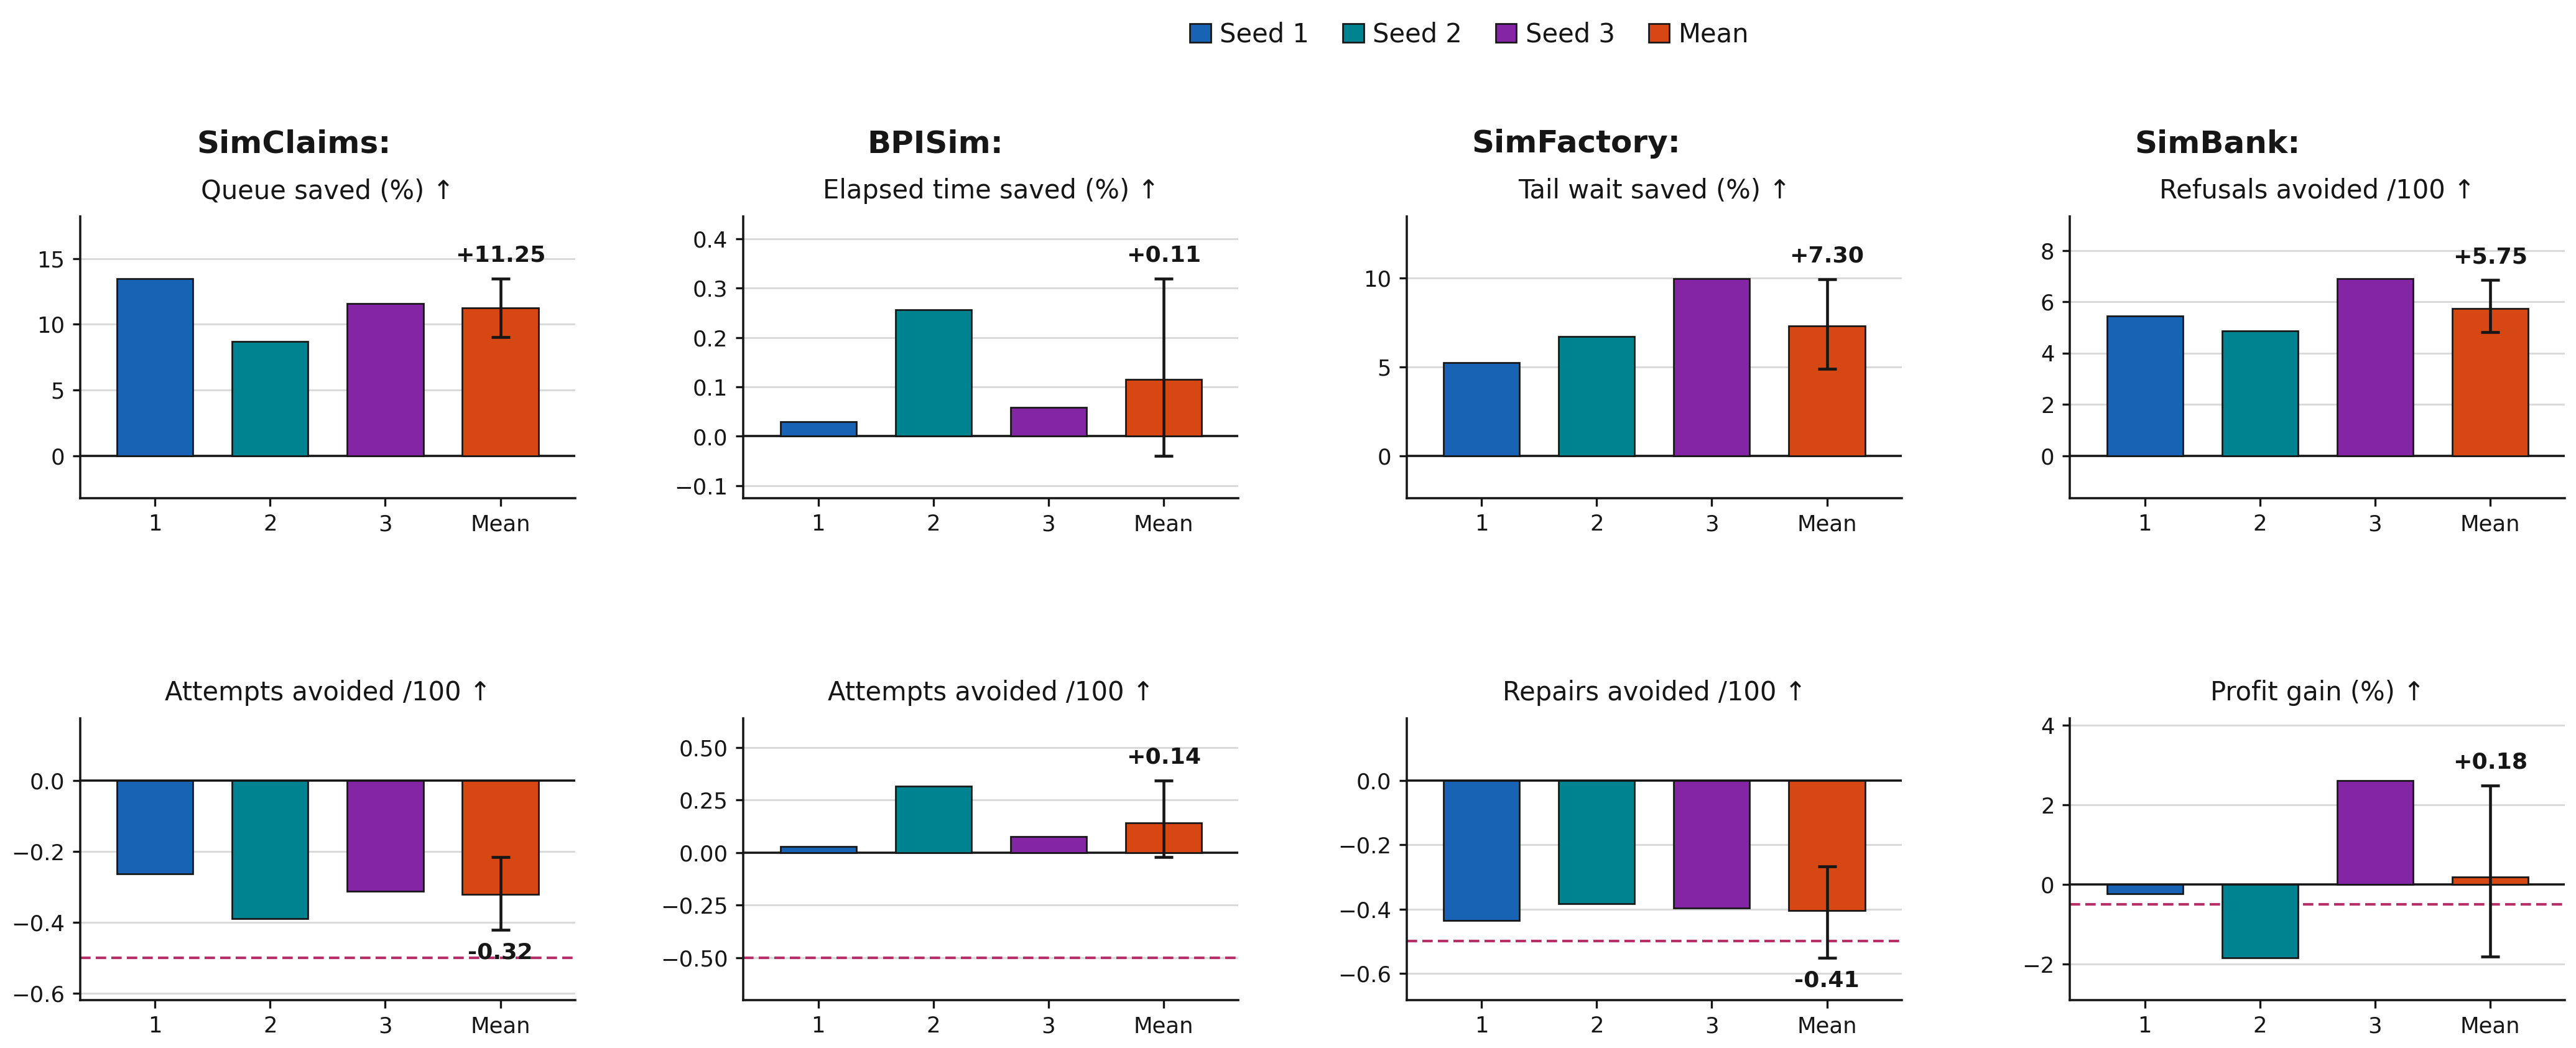
\includegraphics[width=.96\textwidth]{img/fig03_focused_results.png}
\caption{Seed level gains for the focused Regression based comparisons. BPISim shows the episodic controller sensitivity. Top panels show primary outcomes. Bottom panels show repeat or profit effects. Bars show three random seeds and their mean. Error bars show paired 95\% intervals. Dashed lines mark the declared lower limits.}
\label{fig:tradeoffs}
\end{figure*}

\section{Ablation Studies}
\label{sec:ablations}

Fig.~\ref{fig:tradeoffs} shows the three seed effects for the focused comparisons. Claims, factory and bank improve on their primary outcomes in every seed. The BPISim results remain close to zero. Table~\ref{tab:ablations} then tests which state, objective and data choices explain these results. Positive saved or avoided values favor the first policy in each comparison.

\subsection{Routing Controls and Stress Tests}

In SimClaims, episodic search adds only 0.34 queue minutes [$-0.33$, 0.95] beyond an equally tuned static policy (Table~\ref{tab:ablations}). Removing congestion costs 11.01 minutes [9.97, 12.00]. Removing the forecast residual or restricting intervention to the first attempt improves queue time slightly. The main source of the claims gain is congestion aware allocation, not a more complex forecast correction.

BPISim validation retains Regression in all seeds. Episodic search gives the small result in Table~\ref{tab:focused}. Reviewer queue and work form only 0.68\% of total elapsed time. The intervention cannot change most of the measured outcome. In SimFactory, accrued wait contributes 8.43 saved minutes [1.35, 16.00]. A tail specific reward does not beat the mean queue reward. Under burst arrivals, the controller still saves 34.09 minutes [20.89, 48.94] but the relative gain falls to 3.17\%.

\subsection{Rewards and Logged Action Coverage}

In SimBank, adding refusal and cancellation penalties avoids 2.79 refusals per 100 cases [2.22, 3.51] against profit only CQL. The paired profit change of $-5.70$ units [$-26.69$, 13.30] is unresolved. Forecast features add 71.30 profit units [40.63, 100.20] over history only CQL and avoid 3.20 further refusals per 100 cases. These two ablations support the focused reward and state design.

Ensembling fitted Q adds 7.92 profit units [$-4.75$, 20.42], which is not confirmed. Training from logs dominated by the bank policy reduces profit by 93.77 units [$-152.30$, $-6.27$] against randomized logs. Logged action coverage has a material effect on the offline policy. Native simulator evaluation is needed because off policy estimates alone can be unstable \cite{ope}.

\subsection{Cross Domain Interpretation}

Sequential control improves a strong supervised policy only when its state and reward match the mechanism behind the target metric. Congestion state drives the SimClaims gain. Accrued wait matters in SimFactory. Forecast features and process penalties matter in SimBank. Generic Q learning, CQL or PPO without this alignment does not beat Regression routing.

The gains carry different costs. SimClaims and SimFactory allow small increases in corrective attempts. SimBank reduces repeated refusals without a confirmed profit change. BPISim changes too little of total elapsed time to show a reliable effect. This null result identifies a limit of the intervention, not only a limit of training.

\clearpage
\begin{table*}[!t]
\caption{Component, timing, reward and logging ablations on held out streams.}
\label{tab:ablations}
\centering\fontsize{6.5}{7.1}\selectfont
\setlength{\tabcolsep}{4pt}
\renewcommand{\arraystretch}{0.92}
\begin{tabularx}{\textwidth}{@{}L{2.35in}L{1.55in}Y@{}}
\toprule
Domain and question & Comparison & Held out result [95\% CI] \\
\midrule
\textit{SimClaims:} Does search add to equal static tuning? & Full vs. equal static & $0.34\;[-0.33,\,0.95]$ queue min saved. No confirmed residual gain. \\
\textit{SimClaims:} Is congestion state useful? & Full vs. no congestion & $11.01\;[9.97,\,12.00]$ queue min saved. Congestion is essential. \\
\textit{SimClaims:} Do forecast residuals help? & Full vs. no forecast & $-0.65\;[-1.26,\,-0.11]$ queue min saved. Forecast residuals reduce queue performance. \\
\textit{SimClaims:} Do later repeat decisions help? & Full vs. first only & $-0.62\;[-1.39,\,-0.06]$ queue min saved. First only routing is better. \\
\midrule
\textit{BPISim:} Does validation select search? & Selected vs. Regression & $0.00\;[0.00,\,0.00]$ elapsed min saved. Regression is selected for all seeds. \\
\textit{BPISim:} Can episodic search improve elapsed time? & Episodic search vs. Regression & $10.32\;[-3.55,\,28.66]$ elapsed min saved. The gain is not confirmed. \\
\textit{BPISim:} How much elapsed time can review affect? & Review queue and work share & $0.68\%$ of elapsed time. Most elapsed time is outside the decision. \\
\midrule
\textit{SimFactory:} Does accrued waiting state help? & Safe vs. no accrued wait & $8.43\;[1.35,\,16.00]$ tail min saved. Accrued wait is useful. \\
\textit{SimFactory:} Does the tail reward beat mean queue reward? & Tail vs. mean queue objective & $-7.10\;[-17.67,\,4.96]$ tail min saved. No confirmed advantage. \\
\textit{SimFactory:} Does the gain survive burst arrivals? & Safe vs. Regression under bursts & $34.09\;[20.89,\,48.94]$ tail min saved $(3.17\%)$. The gain remains below the 5\% target. \\
\midrule
\textit{SimBank:} Do process penalties reduce refusals? & Both penalties vs. profit only & $2.79\;[2.22,\,3.51]$ refusals avoided/100. $-5.70\;[-26.69,\,13.30]$ profit change. \\
\textit{SimBank:} Do forecast features help CQL? & Full vs. history only CQL & $71.30\;[40.63,\,100.20]$ profit change. $3.20\;[1.94,\,4.21]$ refusals avoided/100. \\
\textit{SimBank:} Does ensembling improve fitted Q? & Ensemble vs. single model & $7.92\;[-4.75,\,20.42]$ profit change. The gain is not confirmed. \\
\textit{SimBank:} Does biased logging change the policy? & Biased vs. random logs & $-93.77\;[-152.30,\,-6.27]$ profit change. Biased logs reduce profit. \\
\bottomrule
\end{tabularx}
\par\smallskip
\begin{minipage}{\textwidth}\fontsize{6.5}{7.1}\selectfont
Positive saved or avoided values favor the first policy. Profit change is first minus second. Intervals are paired across three random seeds. The review share is descriptive.
\end{minipage}
\end{table*}

\FloatBarrier

\section{Discussion}
\label{sec:discussion}

The repeated events have different meanings. Manufacturing repair includes explicit reinspection and gives the clearest physical rework signal. A later document request may be routine. A refused offer is a repeated decision, not corrective work. We keep these domain outcomes separate.

\textit{Limitations:} Claims service time is a proxy. SimFactory has few later repairs for historical checking. Staffing, difficulty and specialist effects are scenario inputs. The results support comparisons inside the declared simulators, not causal claims for the source organizations.

\section{Conclusion}
\label{sec:conclusion}

This work connects models of rework, loops and repeated decisions with supervised prediction and sequential control. Focused controllers improve claims queue time, manufacturing tail wait and repeated loan refusals against matched Regression policies. BPISim shows no reliable elapsed time gain because review forms little of turnaround. Control adds value when its state and reward match the process bottleneck. Repeat and profit effects remain part of that result.

\noindent Code: \url{https://github.com/WhiteMetagross/LoopLab}

\FloatBarrier
\bibliographystyle{IEEEtran}
\bibliography{references}

\end{document}
